\providecommand{\myrootdir}{..}
\documentclass[\myrootdir/main.tex]{subfiles}

\begin{document}

\chapter{Empirical Comparison Study}
\label{sec:study}
To investigate how different factors \todo{do we list these somewhere?} influence BLIRTs we evaluate the three techniques implemented in our tool on the \emph{Failing Build Log Data Set}.

\begin{figure}[htbp]
	\centering
	\includegraphics[page=6, width=\textwidth, trim={0.5cm 0.5cm 0.5cm 0.5cm}, clip]{img/flow-of-research.pdf}
	\caption{Process of our technique comparison study}
	\label{fig:study}
\end{figure}

\section{Study Design}
\bp{We compare three different techniques: PBE, TS, SKWS (itemize and link to their explanation?) and as a baseline: random line rerieval (RLR): retrieves random lines from the build log, (describe in chapper about BLIRTs??), number of lines: average of output lines from past}
We configure the technique for every example set with an increasing count of I/O examples and then run the retrieval on the next I/O example, the \emph{test I/O example}.
The output from the test I/O example is the oracle for our evaluation.
The examples are sorted and selected chronologically, i.e. the technique is configured with examples from the directly preceeding build logs to extract information from the test log.
The extraction quality of a BLIRT run is evaluated on only one build log, as it should be suitable for every coming example.
Especially the one directly succeeding the configuration.
If the information retrieval there is bad, we expect the user to directly change the configuration again or be dissapointed with his selection of technique.

When evaluating a BLIRT run we measure the following data points:
\begin{itemize}
	\item \textbf{Successful} A BLIRT run is successful when the retrieved output contains all the lines the oracle output.
	\item \textbf{Accuracy} \todo{currently: levenstein difference of input and output, maybe: change to false pos and neg lines}
	\item \textbf{Proximity} \todo{No! let's do that with "}
\end{itemize}

taking The Failing Build Log Data Set - run 3(4 with random) techniques with increasing example count - measuring xyz - justify choices like running chronologically / testing on 1 example / no k-fold validation - how are keywords for the search selected?

\section{Results}

\begin{figure}[htbp]
	\centering
	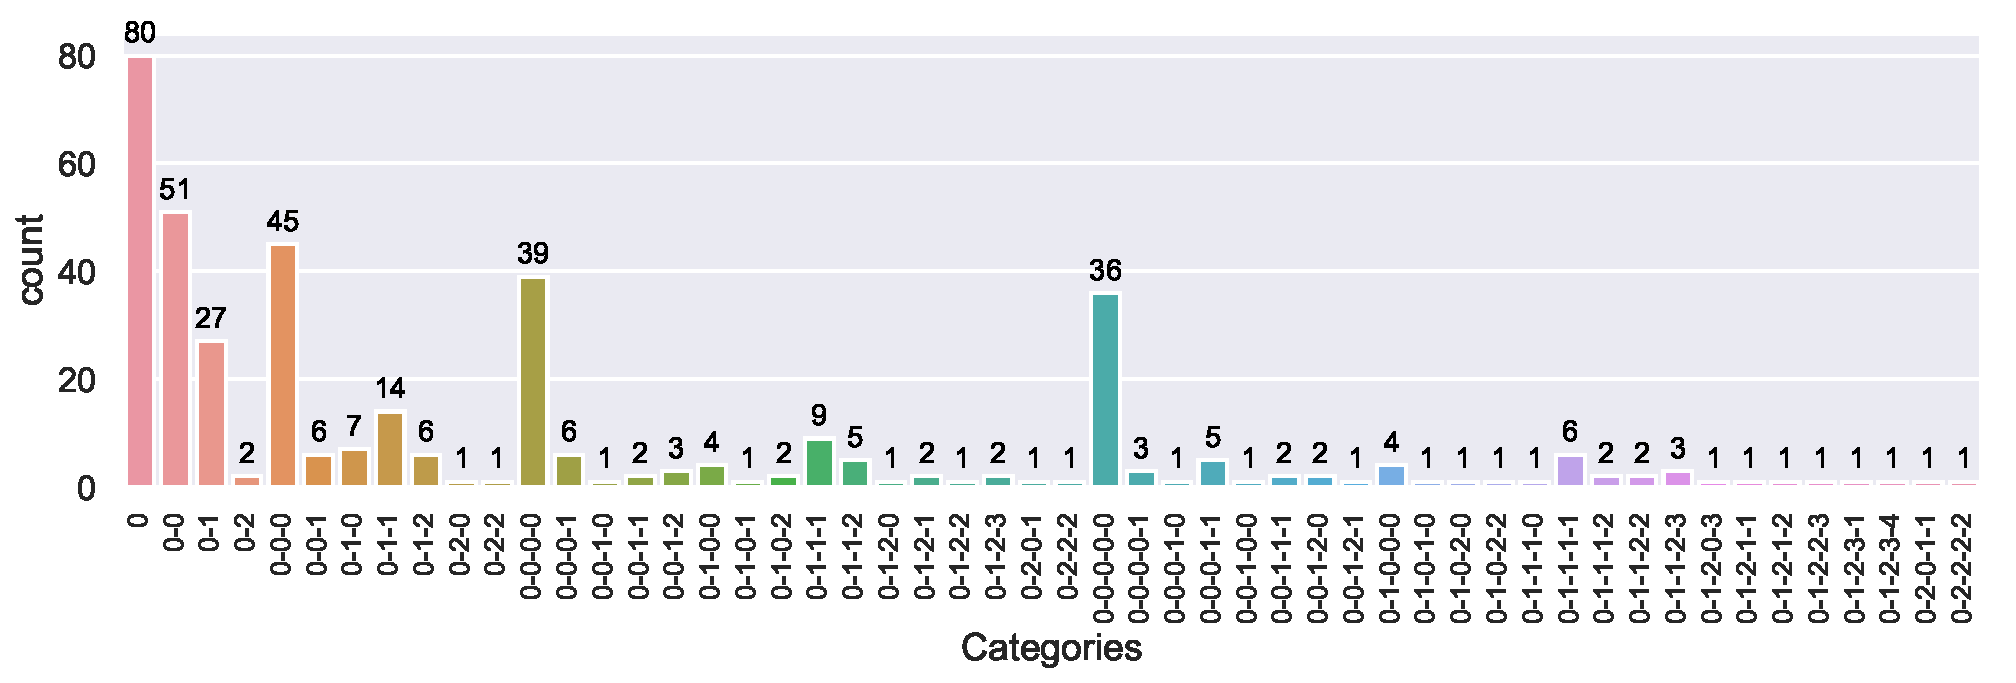
\includegraphics[width=\textwidth, clip]{img/big-study/categories-dataset.pdf}
	\caption{Distribution of Category Combinations in the Example Sets used for Configuration in our Study}
	\label{fig:categories-dataset}
\end{figure}

\begin{figure}[htbp]
	\centering
	\begin{minipage}{0.45\textwidth}
		\centering
		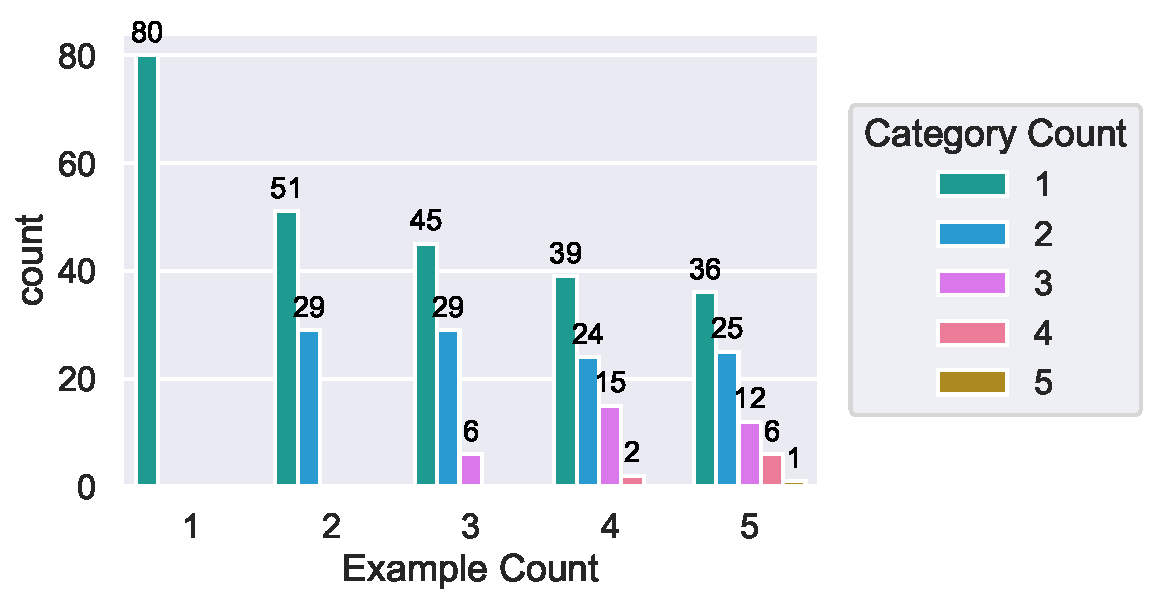
\includegraphics[width=\textwidth, clip]{img/big-study/categorycount-examplecount-dataset.pdf}
		\caption{Distribution of the Count of Categories within the Examples used for Configuration in our Study}
		\label{fig:categorycount-examplecount-dataset}
	\end{minipage}\hfill
	\begin{minipage}{0.45\textwidth}
		\centering
		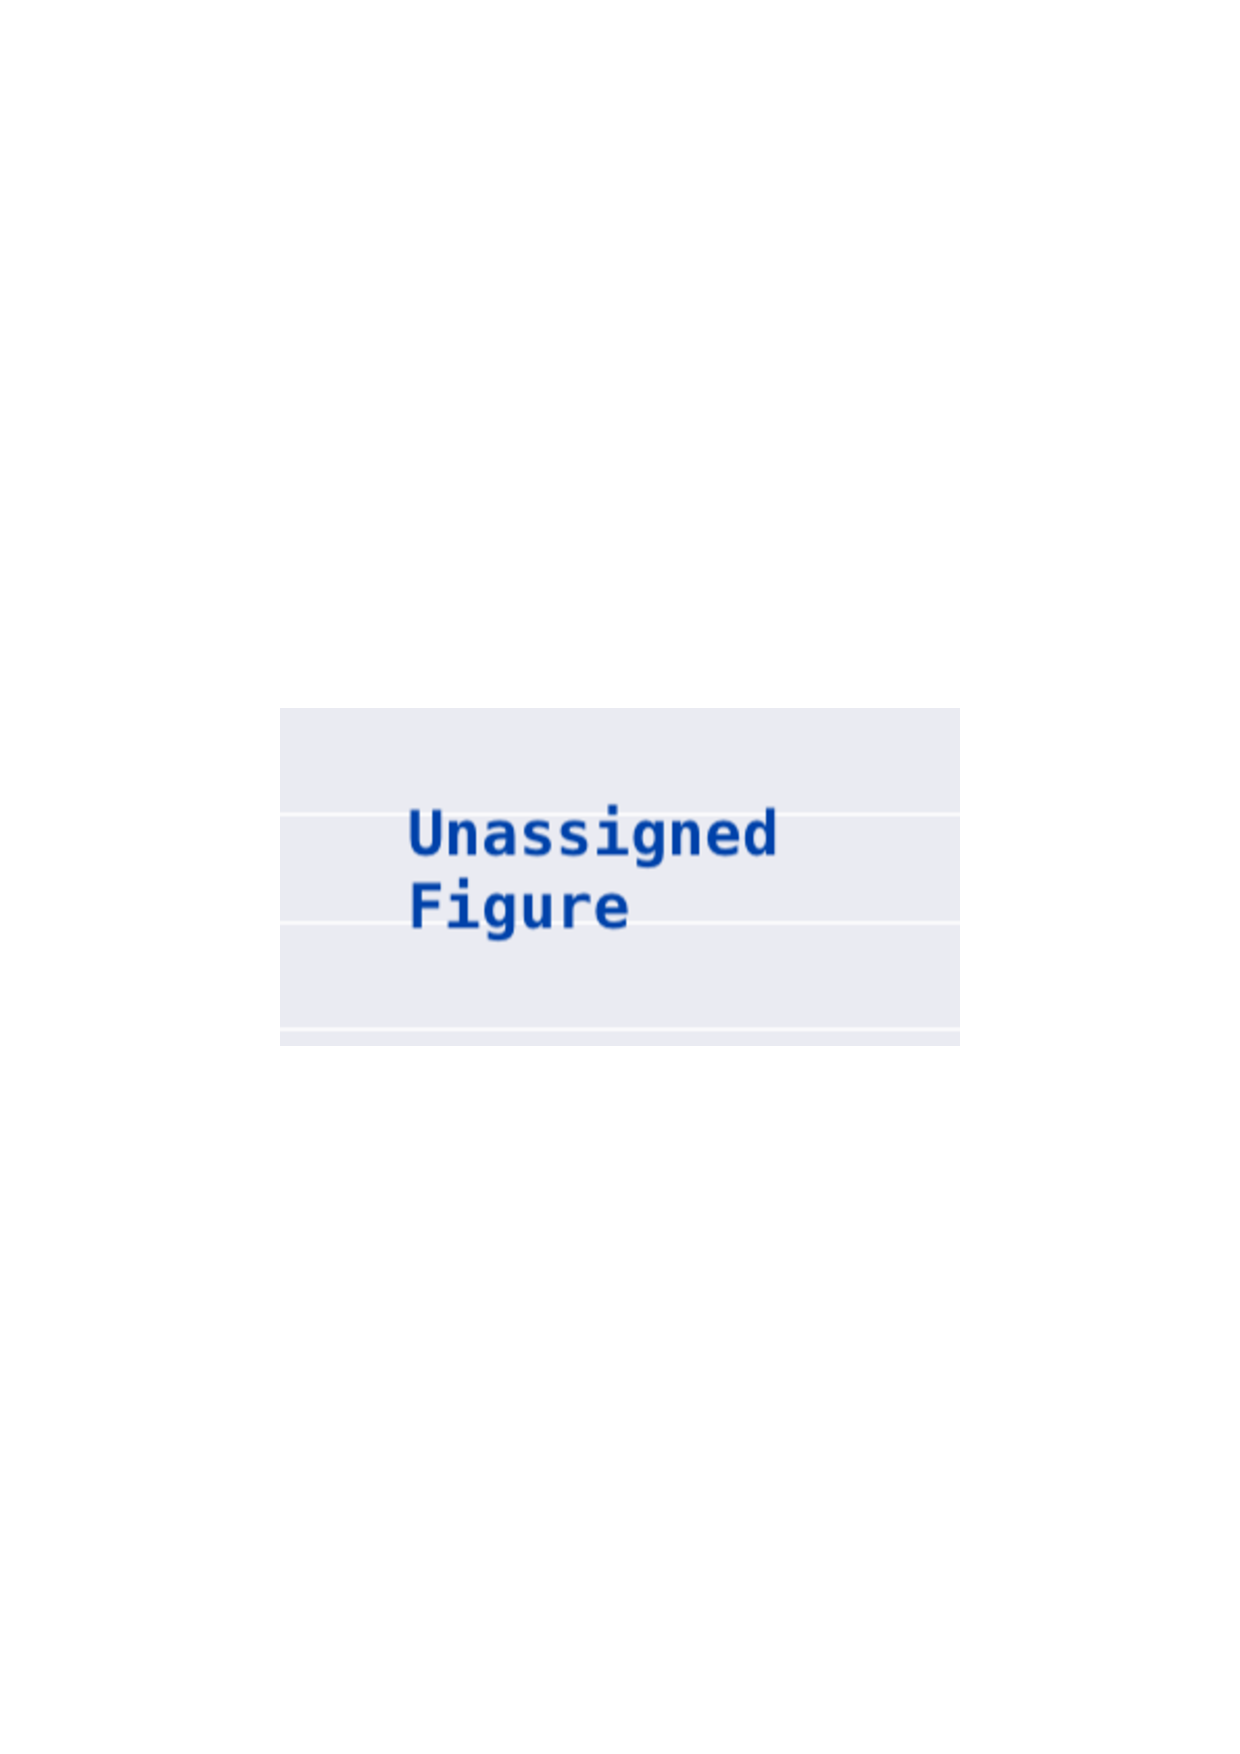
\includegraphics[width=\textwidth, clip]{img/big-study/xxx.pdf}
		\caption{caption}
		\label{fig:xxxy}
	\end{minipage}
\end{figure}

\subsection{Category Distribution in Data Set}
Categories distributed in over data set
- why are we looking at that?: interesting how categories are distributed for this real world example of build Failure reasons in travis ci categorization
- Figure \ref{fig:categories-dataset} shows the distribution of categories in the configuring example sets in rou study
- Figure \ref{fig:categorycount-examplecount-dataset} shows the category count separated by the different example count.


\subsection{Regular Expression Program Synthesis by Example (PBE)}

\begin{figure}[htbp]
	\centering
	\begin{minipage}{0.45\textwidth}
		\centering
		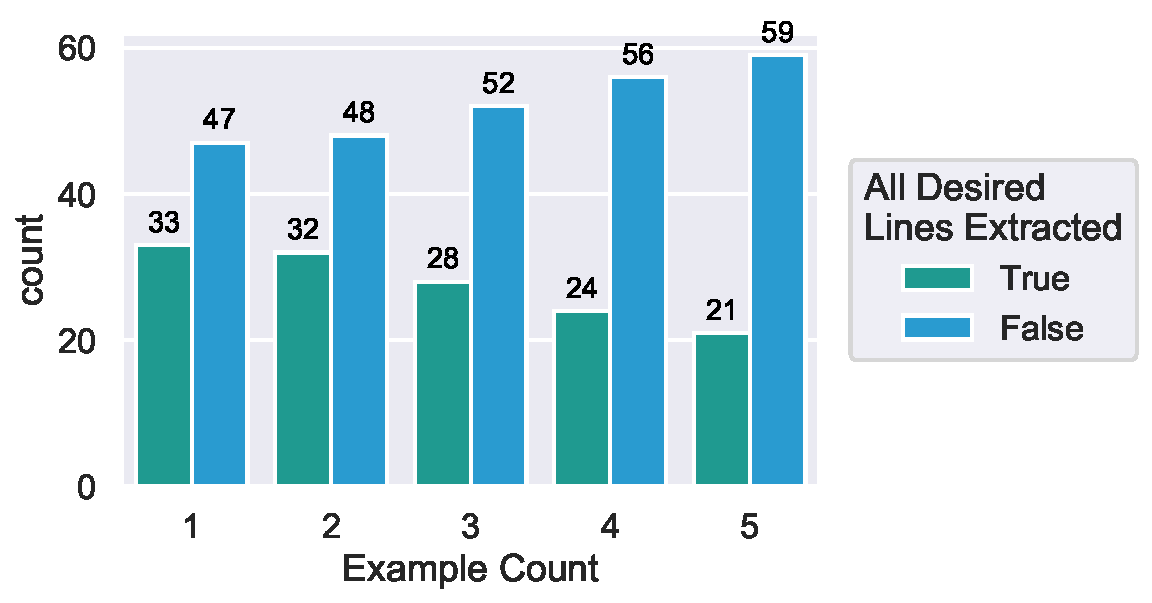
\includegraphics[width=\textwidth, clip]{img/big-study/success-examples-PBE.pdf}
		\caption{Successful Extractions per Number of Examples for PBE}
		\label{fig:success-examples-pbe}
	\end{minipage}\hfill
	\begin{minipage}{0.45\textwidth}
		\centering
		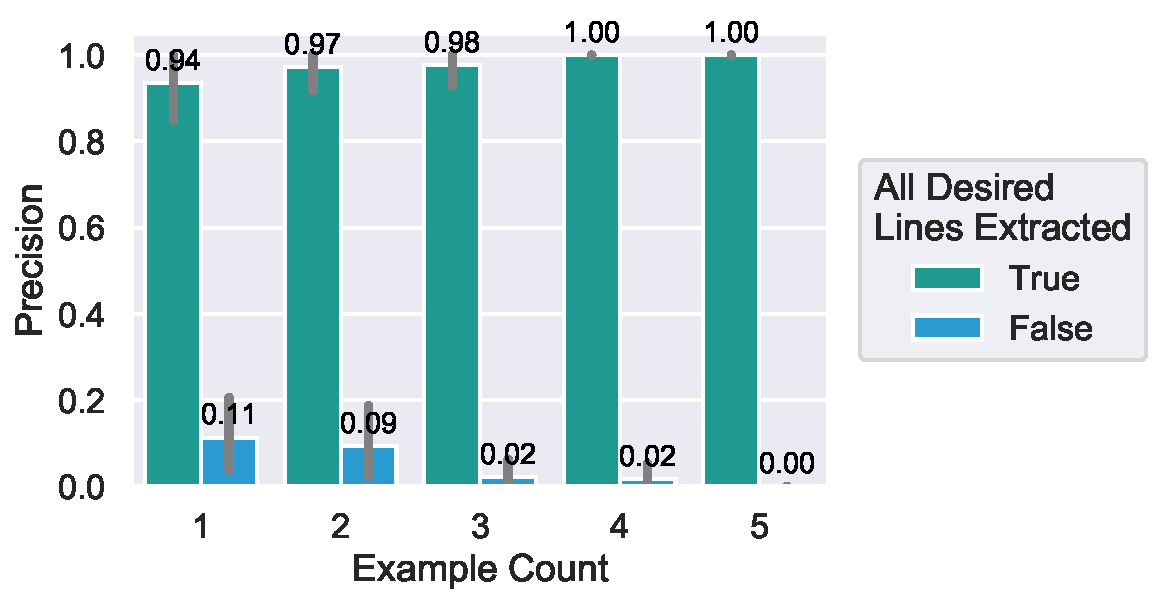
\includegraphics[width=\textwidth, clip]{img/big-study/precision-PBE.pdf}
		\caption{Precision of Extractions per Number of Examples for PBE}
		\label{fig:precision-pbe}
	\end{minipage}
\end{figure}
\begin{figure}[htbp]
	\centering
	\begin{minipage}{0.45\textwidth}
		\centering
		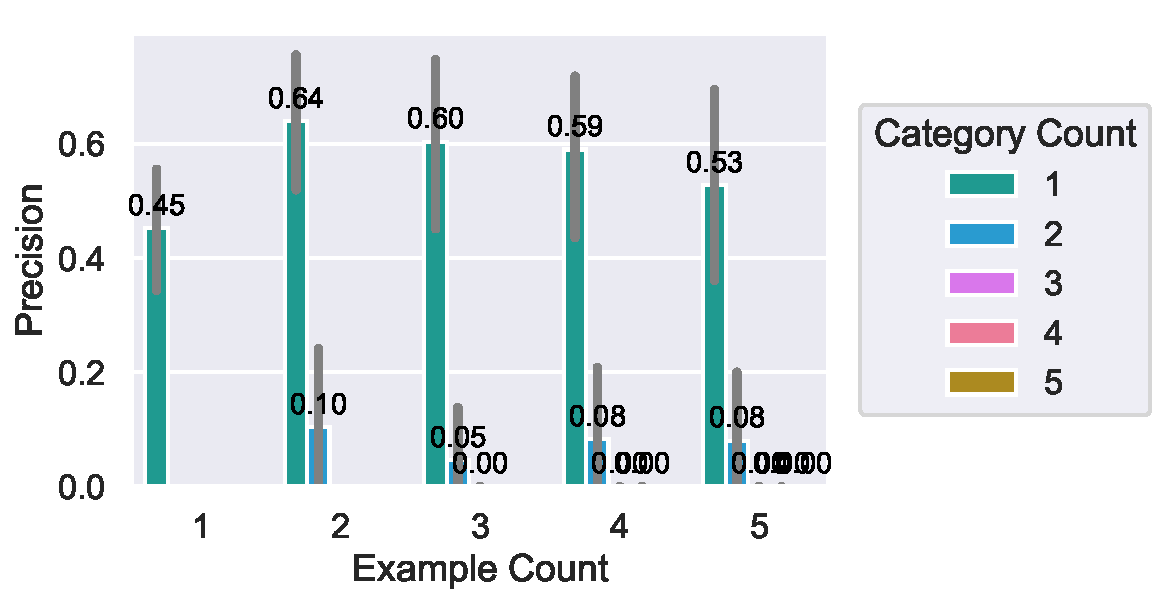
\includegraphics[width=\textwidth, clip]{img/big-study/precision-categorycount-examplecount-PBE.pdf}
		\caption{Precision of PBE Extractions by CategoryCount}
		\label{fig:precision-categorycount-examplecount-pbe}
	\end{minipage}\hfill
	\begin{minipage}{0.45\textwidth}
		\centering
		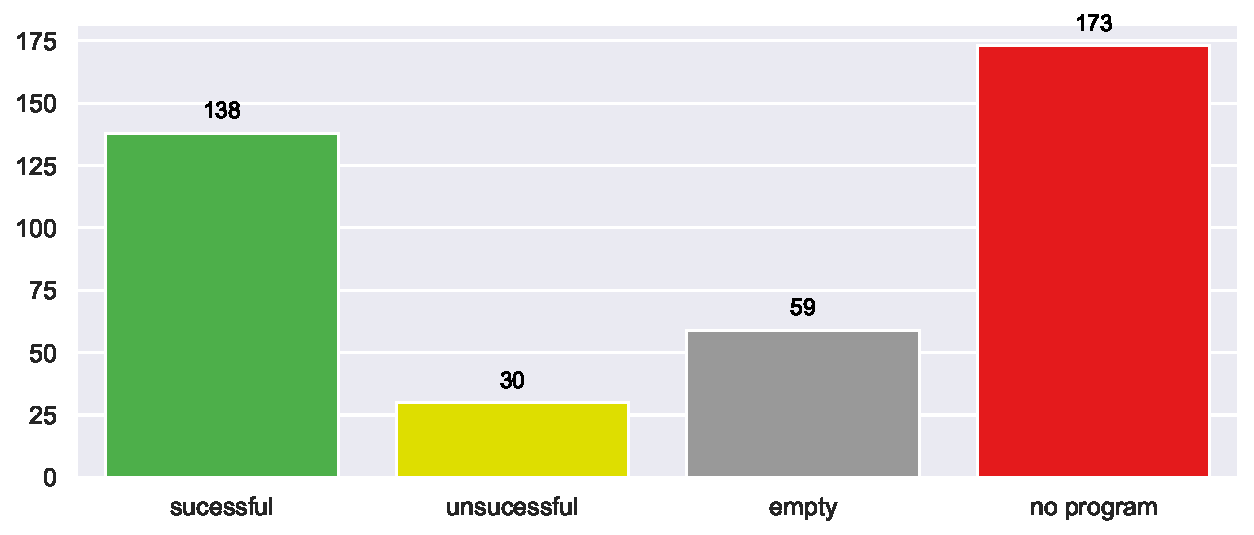
\includegraphics[width=\textwidth, clip]{img/big-study/failure-reason-PBE.pdf}
		\caption{Reasons for PBE Runs to Fail}
		\label{fig:failure-reason-pbe}
	\end{minipage}
\end{figure}

This section addresses the results produced by the PBE technique in our study.
We start by comparing success rate and precision for different example counts and showing the influence of example categories.
Next we go into detail in which cases pbe fails
\subsubsection{Success-Rate}
\subsubsection{Precision}
\subsubsection{Example Categories}
\subsubsection{Specific Failure Reasons}
\todo{FAILURE REASON AGAINST EXAMPLE CATEGORIES}
% \subsection{Successful Extractions}
% successful is interpreted by us as: all lines that were desired (within our oracle) were also extracted during the test

% Figure \ref{fig:success-all} shows how successful the four different tecnhiques were in our study.
% Figure \ref{fig:success-examples-pbe} shows that the success rate for PBE decreases with increasing example count for pbe. Section \ref{TODO ref to pbe section} explains in more detail whi this fails
% Figure \ref{fig:success-examples-ts} shows that the success rate for TS varies but stays roughly the same for different example counts
% Figure \ref{fig:success-examples-skws} shows that the success rate for KWS varies but stays roughly the same for different example counts
% Figure \ref{fig:success-examples-pbe} shows that 

\subsection{Common Text Similarity (CTS)}

\begin{figure}[htbp]
	\centering
	\begin{minipage}{0.45\textwidth}
		\centering
		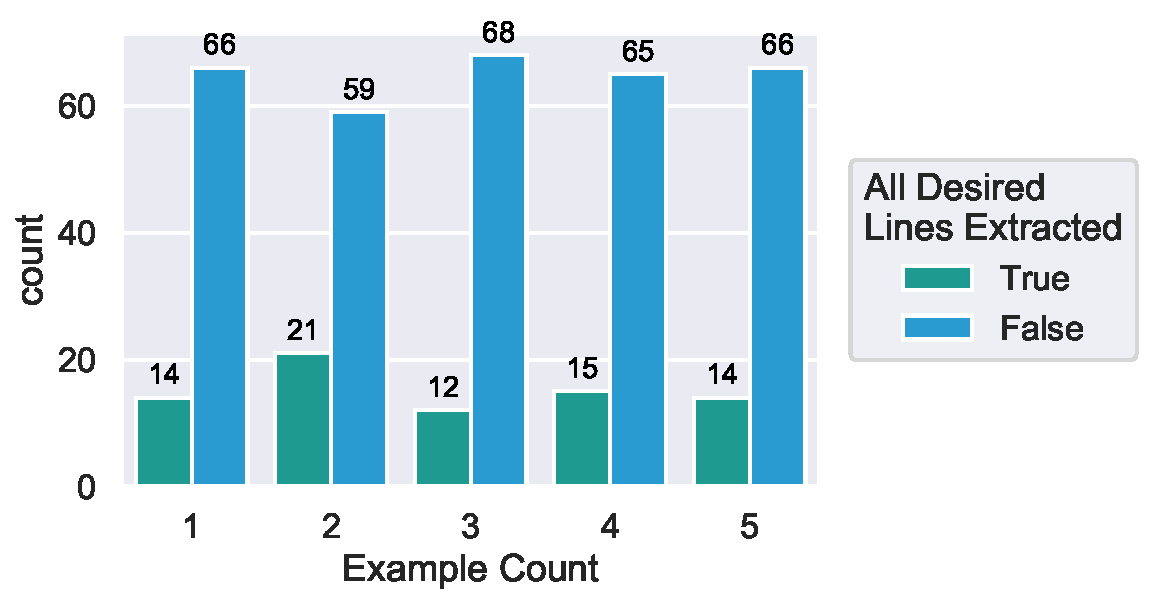
\includegraphics[width=\textwidth, clip]{img/big-study/success-examples-TS.pdf}
		\caption{Successful Extractions per Number of Examples for TS}
		\label{fig:success-examples-ts}
	\end{minipage}\hfill
	\begin{minipage}{0.45\textwidth}
		\centering
		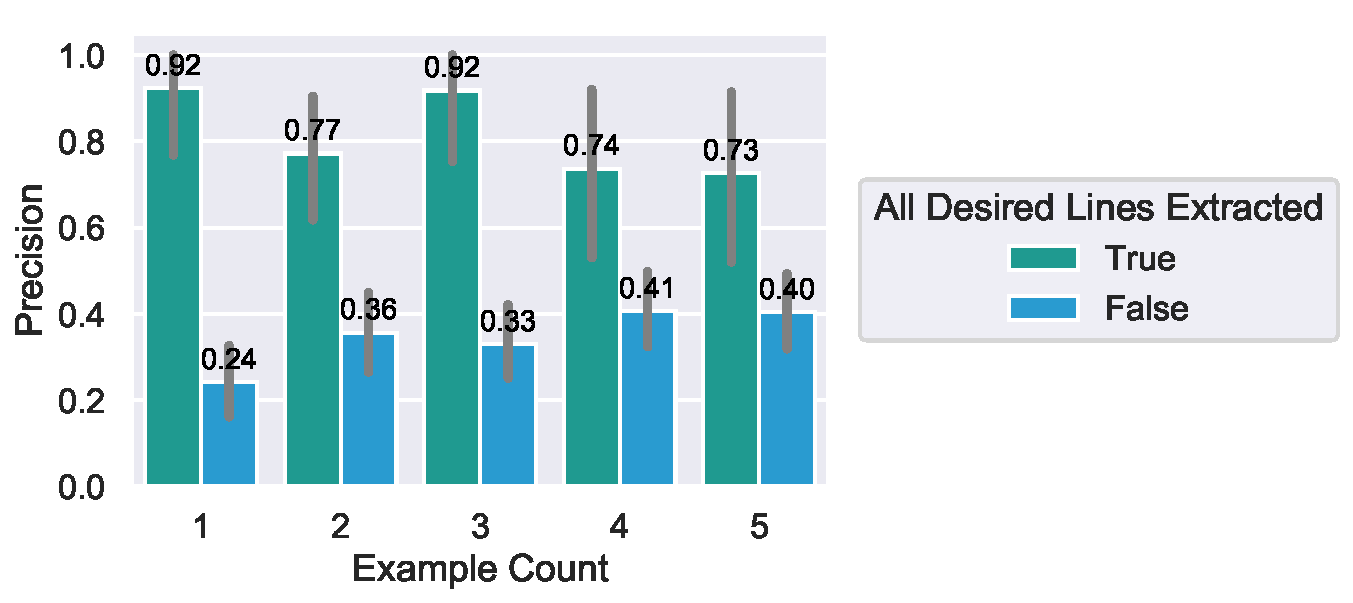
\includegraphics[width=\textwidth, clip]{img/big-study/precision-TS.pdf}
		\caption{Precision of Extractions per Number of Examples for TS}
		\label{fig:precision-ts}
	\end{minipage}
\end{figure}
\begin{figure}[htbp]
	\centering
	\begin{minipage}{0.45\textwidth}
		\centering
		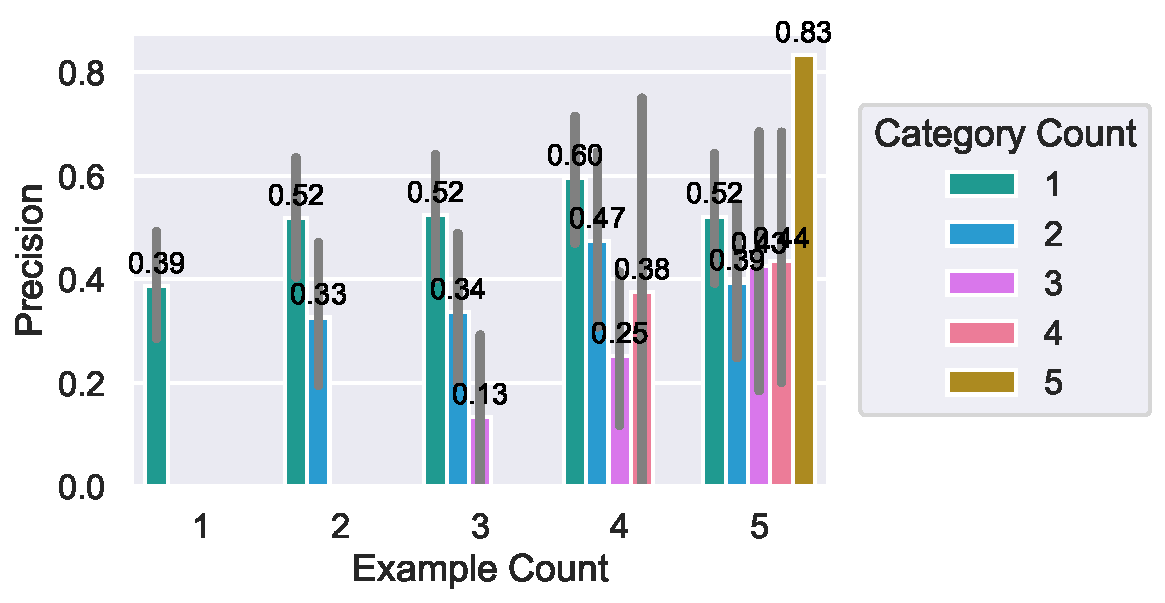
\includegraphics[width=\textwidth, clip]{img/big-study/precision-categorycount-examplecount-TS.pdf}
		\caption{Precision of TS Extractions by CategoryCount}
		\label{fig:precision-categorycount-examplecount-ts}
	\end{minipage}\hfill
	\begin{minipage}{0.45\textwidth}
		\centering
		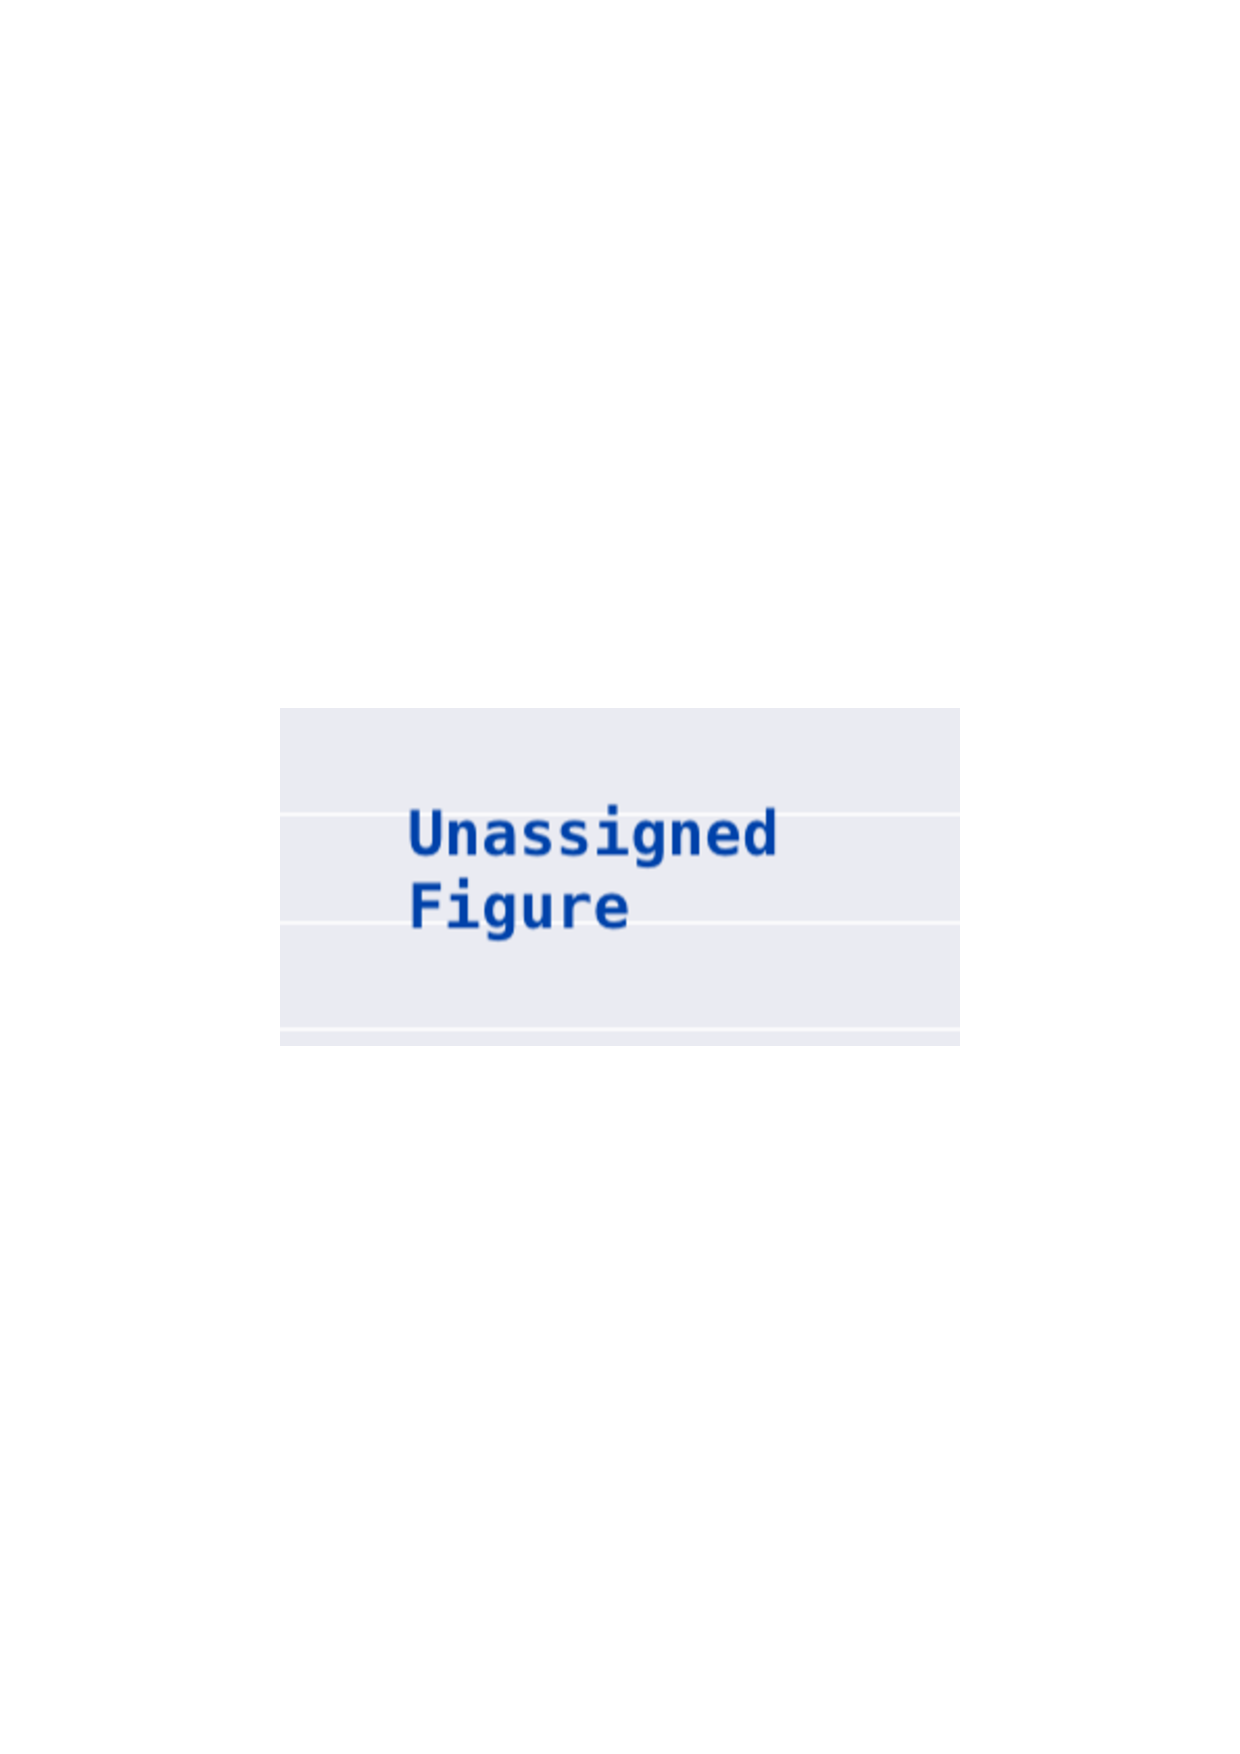
\includegraphics[width=\textwidth, clip]{img/big-study/xxx.pdf}
		\caption{xxx}
		\label{fig:xxx}
	\end{minipage}
\end{figure}

\subsubsection{Success-Rate}
\subsubsection{Precision}
\subsubsection{Example Categories}


\subsection{Keyword Search (KWS)}

\begin{figure}[htbp]
	\centering
	\begin{minipage}{0.45\textwidth}
		\centering
		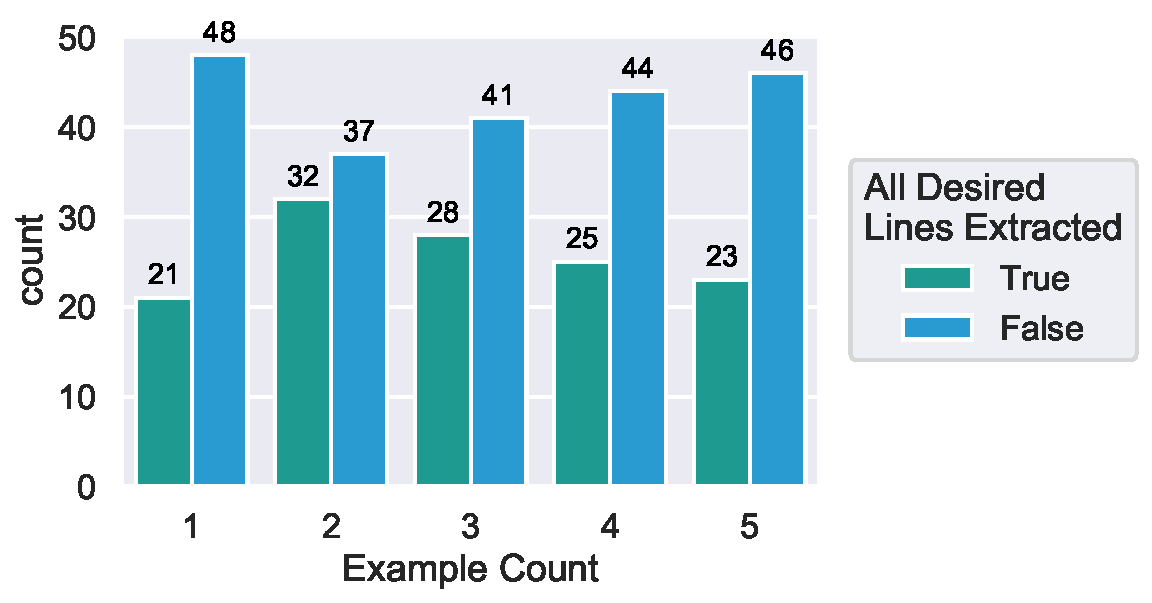
\includegraphics[width=\textwidth, clip]{img/big-study/success-examples-SKWS.pdf}
		\caption{Successful Extractions per Number of Examples for SKWS}
		\label{fig:success-examples-skws}
	\end{minipage}\hfill
	\begin{minipage}{0.45\textwidth}
		\centering
		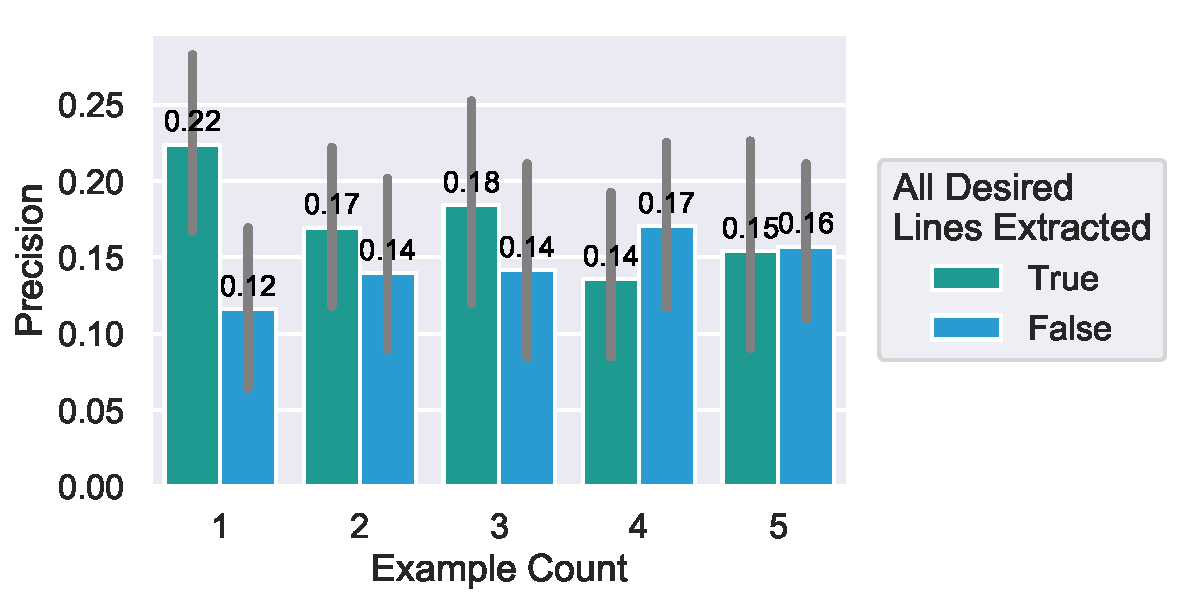
\includegraphics[width=\textwidth, clip]{img/big-study/precision-SKWS.pdf}
		\caption{Precision of Extractions per Number of Examples for SKWS}
		\label{fig:precision-skws}
	\end{minipage}
\end{figure}
\begin{figure}[htbp]
	\centering
	\begin{minipage}{0.45\textwidth}
		\centering
		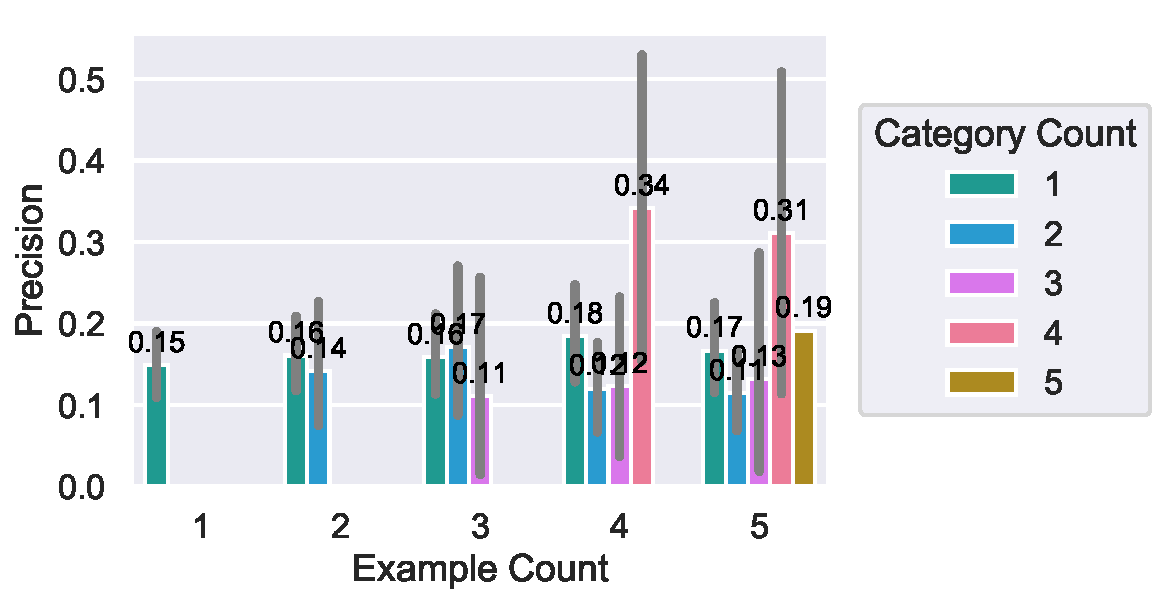
\includegraphics[width=\textwidth, clip]{img/big-study/precision-categorycount-examplecount-SKWS.pdf}
		\caption{Precision of SKWS Extractions by CategoryCount}
		\label{fig:precision-categorycount-examplecount-skws}
	\end{minipage}\hfill
	\begin{minipage}{0.45\textwidth}
		\centering
		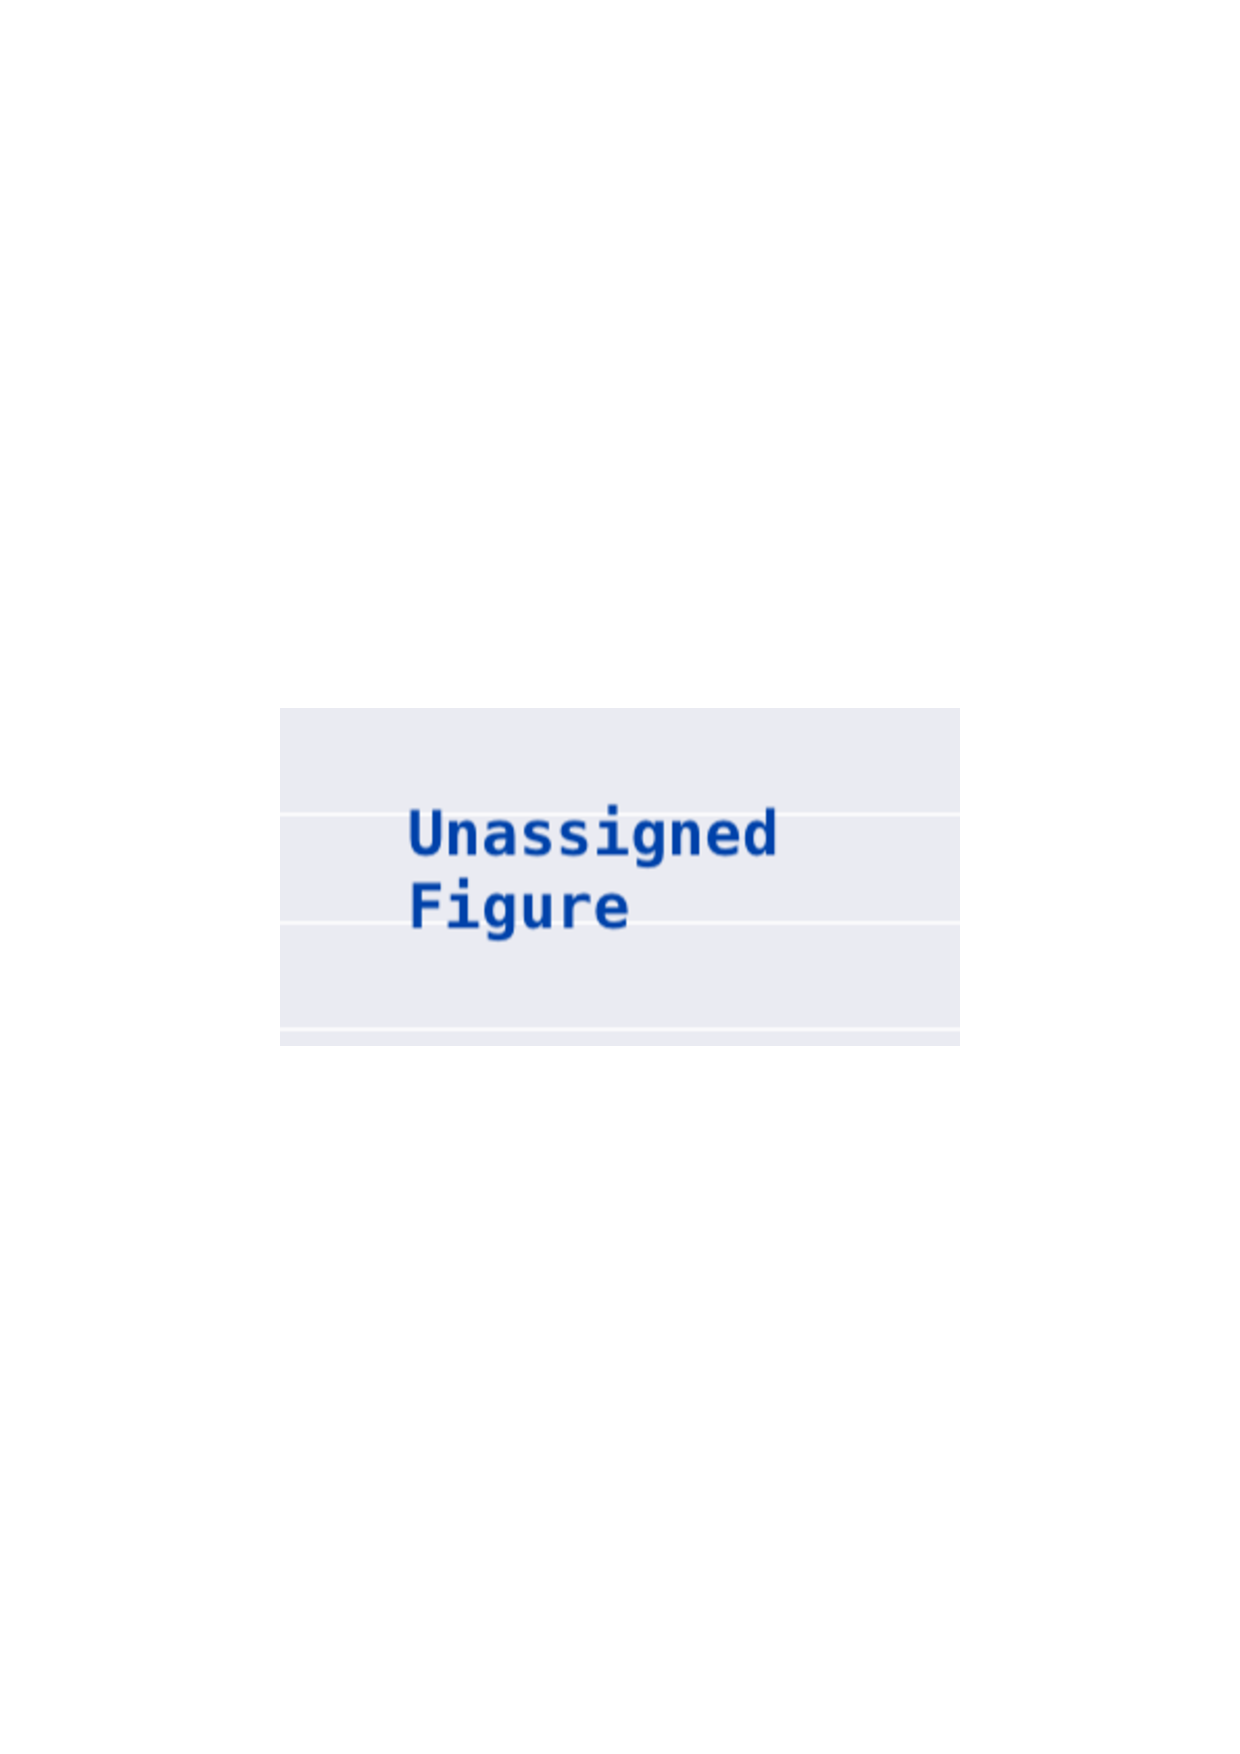
\includegraphics[width=\textwidth, clip]{img/big-study/xxx.pdf}
		\caption{xxx}
		\label{fig:xxx}
	\end{minipage}
\end{figure}

\subsubsection{Success-Rate}
\subsubsection{Precision}
\subsubsection{Example Categories}


% \subsection{Random Line Retrieval (RLR)}

% \begin{figure}[htbp]
% 	\centering
% 	\begin{minipage}{0.45\textwidth}
% 		\centering
% 		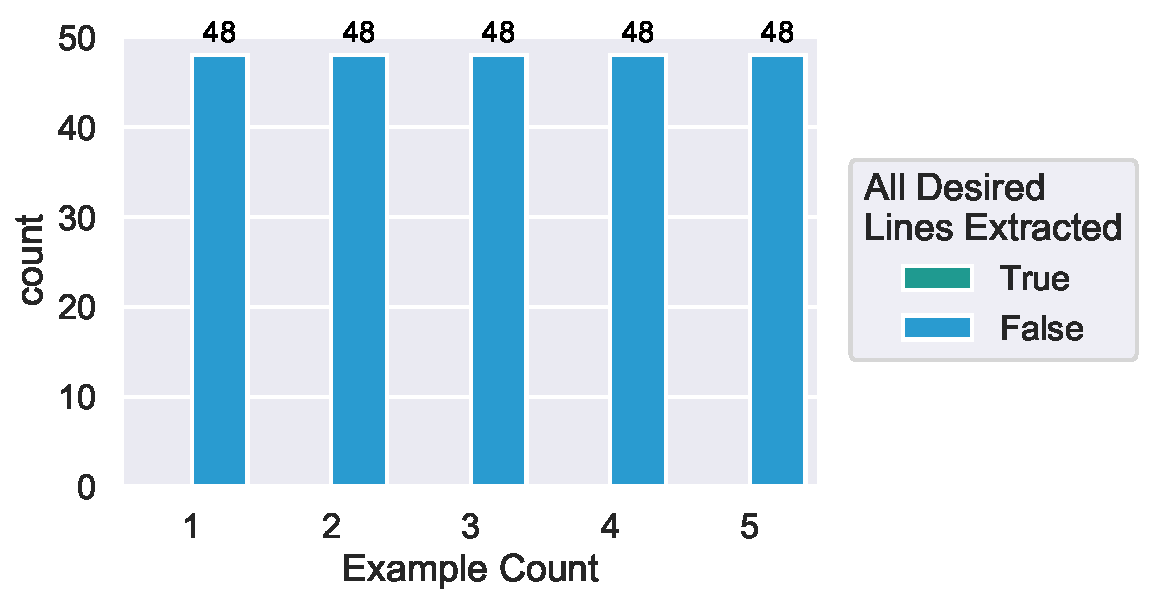
\includegraphics[width=\textwidth, clip]{img/big-study/success-examples-RLR.pdf}
% 		\caption{Successful Extractions per Number of Examples for RLR}
% 		\label{fig:success-examples-rlr}
% 	\end{minipage}\hfill
% 	\begin{minipage}{0.45\textwidth}
% 		\centering
% 		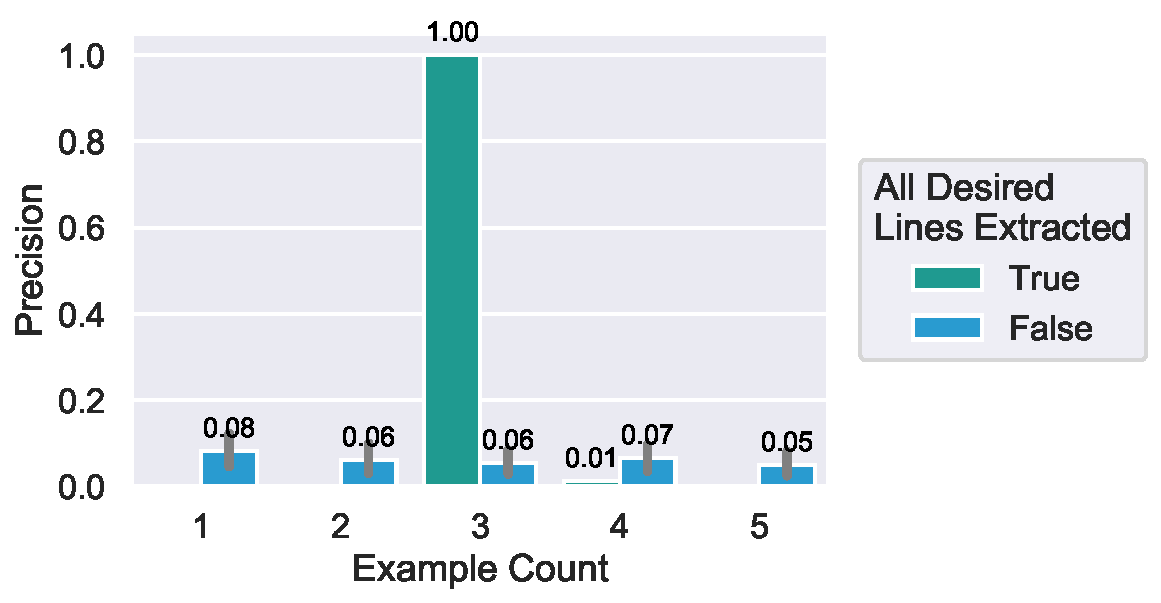
\includegraphics[width=\textwidth, clip]{img/big-study/precision-RLR.pdf}
% 		\caption{Precision of Extractions per Number of Examples for RLR}
% 		\label{fig:precision-rlr}
% 	\end{minipage}
% \end{figure}
% \begin{figure}[htbp]
% 	\centering
% 	\begin{minipage}{0.45\textwidth}
% 		\centering
% 		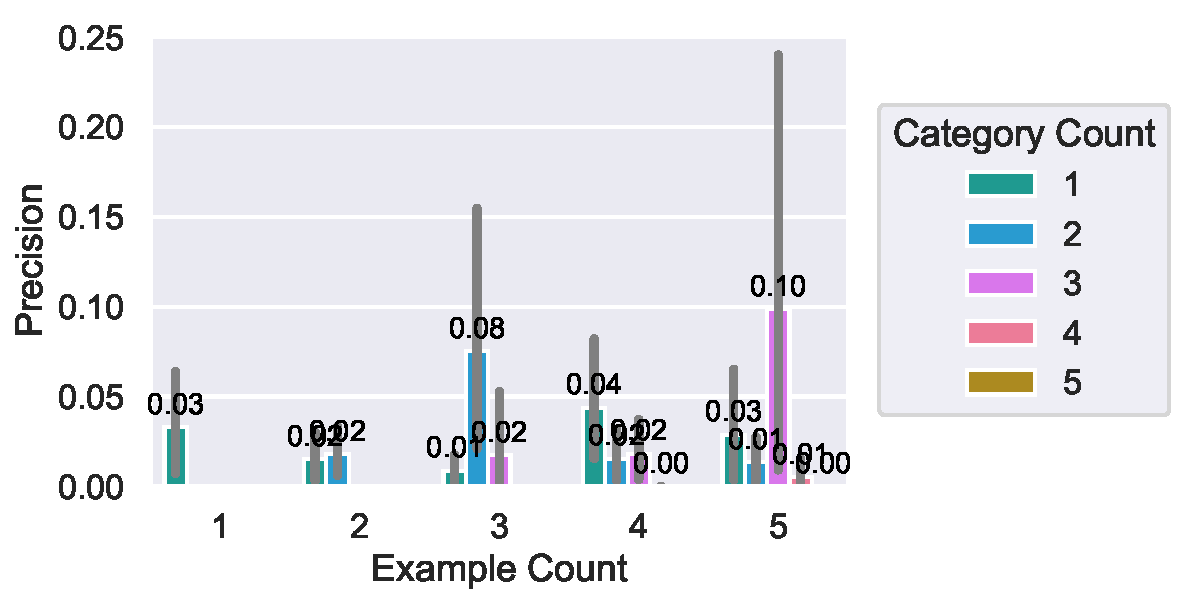
\includegraphics[width=\textwidth, clip]{img/big-study/precision-categorycount-examplecount-RLR.pdf}
% 		\caption{Precision of RLR Extractions by CategoryCount}
% 		\label{fig:precision-categorycount-examplecount-rlr}
% 	\end{minipage}\hfill
% 	\begin{minipage}{0.45\textwidth}
% 		\centering
% 		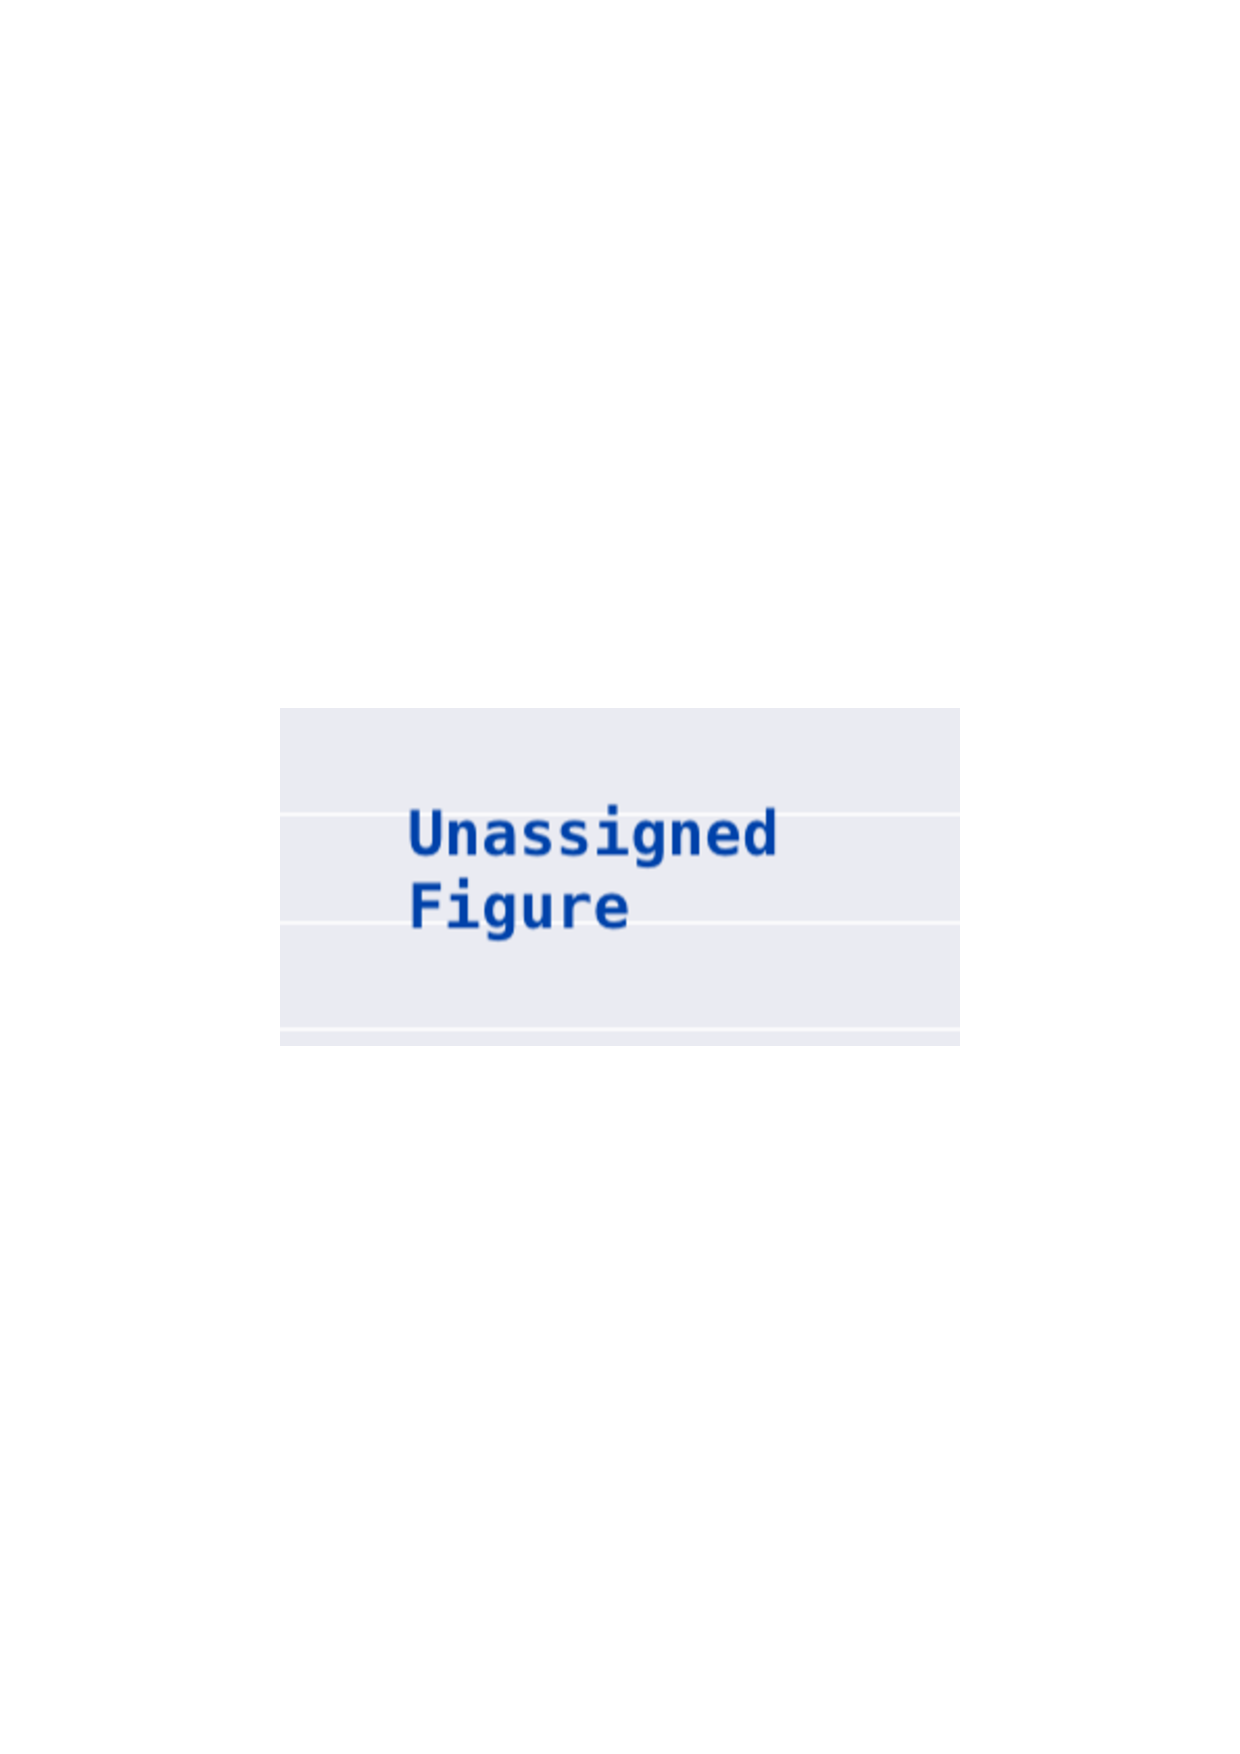
\includegraphics[width=\textwidth, clip]{img/big-study/xxx.pdf}
% 		\caption{xxx}
% 		\label{fig:xxx}
% 	\end{minipage}
% \end{figure}

% For completion this section reports the results for the random line retrieval technique, explained in detail in Section \ref{sec:}

% \subsubsection{Success-Rate}
% \subsubsection{Precision}
% \subsubsection{Example Categories}

\subsection{Comparing All Techniques}
\begin{figure}[htbp]
	\centering
	\begin{minipage}{0.45\textwidth}
		\centering
		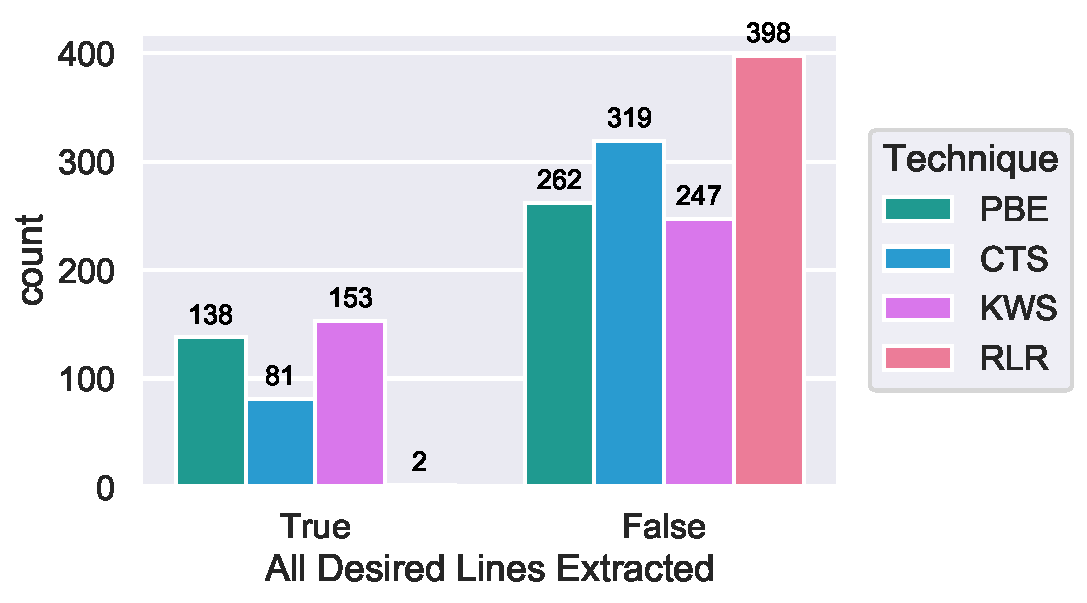
\includegraphics[width=\textwidth, clip]{img/big-study/success-all.pdf}
		\caption{Successful Extractions for all Techniques Compared}
		\label{fig:success-all}
	\end{minipage}\hfill
	\begin{minipage}{0.45\textwidth}
		\centering
		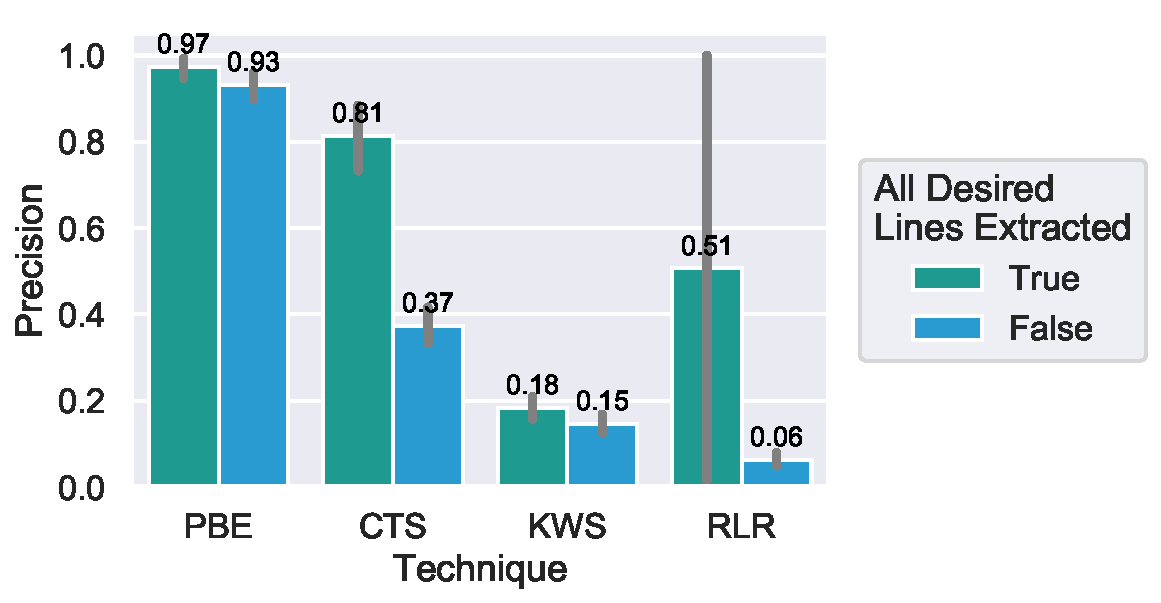
\includegraphics[width=\textwidth, clip]{img/big-study/precision-all.pdf}
		\caption{Precision of Extractions for all Techniques Compared}
		\label{fig:precision-all}
	\end{minipage}
\end{figure}

\begin{figure}[htbp]
	\centering
	\begin{minipage}{0.45\textwidth}
		\centering
		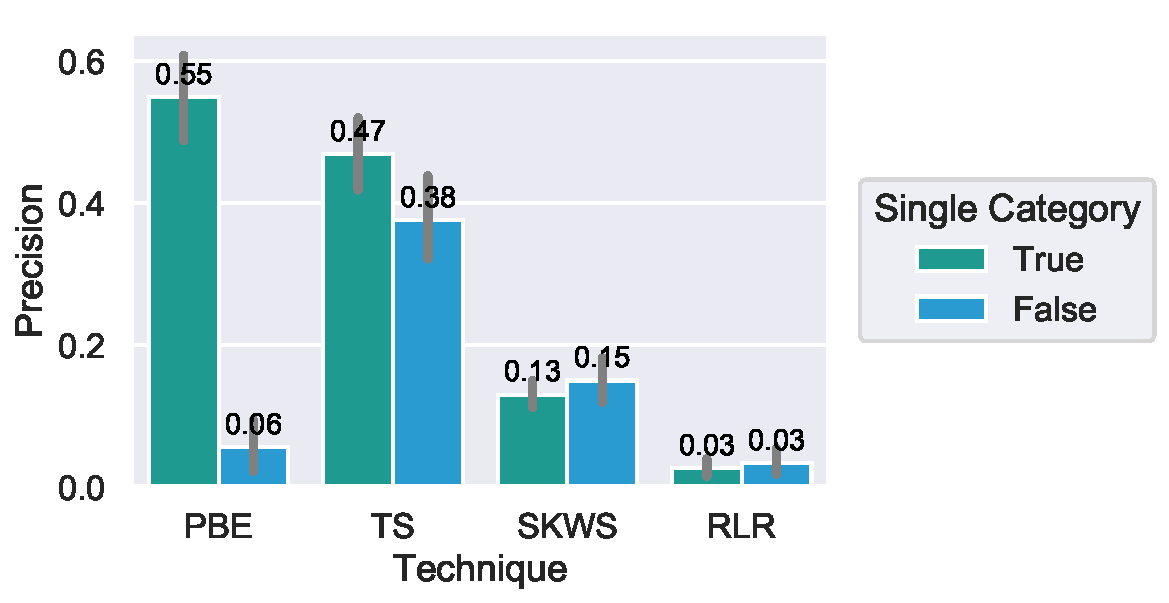
\includegraphics[width=\textwidth, clip]{img/big-study/precision-category-singularity-all.pdf}
		\caption{\todo{todo}}
		\label{fig:precision-category-singularity-all}
	\end{minipage}\hfill
	\begin{minipage}{0.45\textwidth}
		\centering
		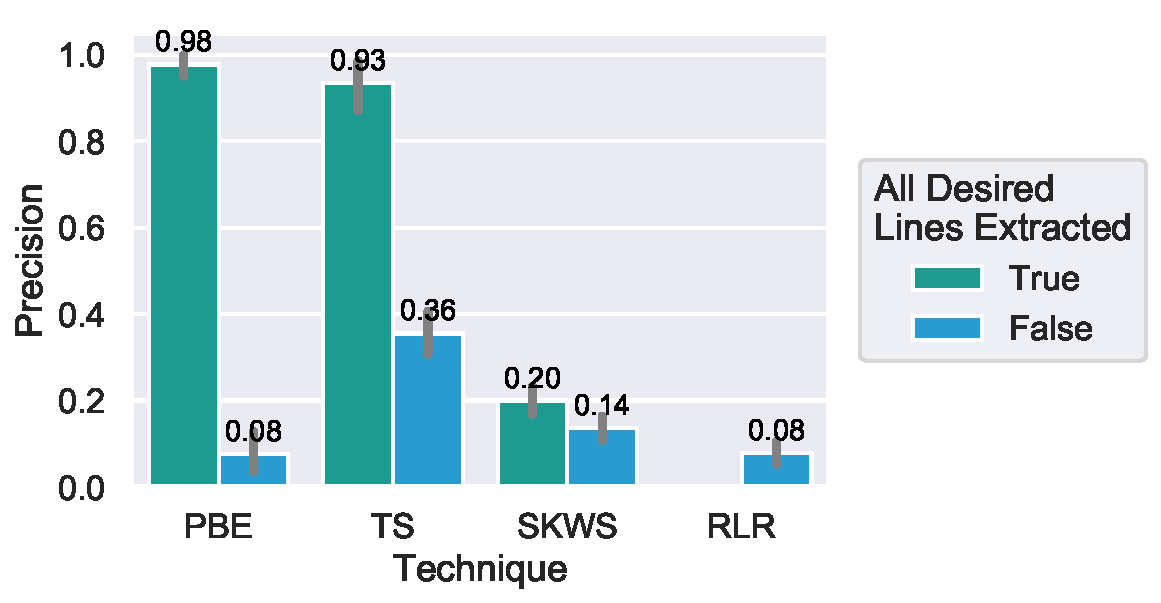
\includegraphics[width=\textwidth, clip]{img/big-study/single-cateogry-precision-all.pdf}
		\caption{\todo{todo}}
		\label{fig:single-cateogry-precision-all}
	\end{minipage}
\end{figure}

\begin{figure}[htbp]
	\centering
	\begin{minipage}{0.45\textwidth}
		\centering
		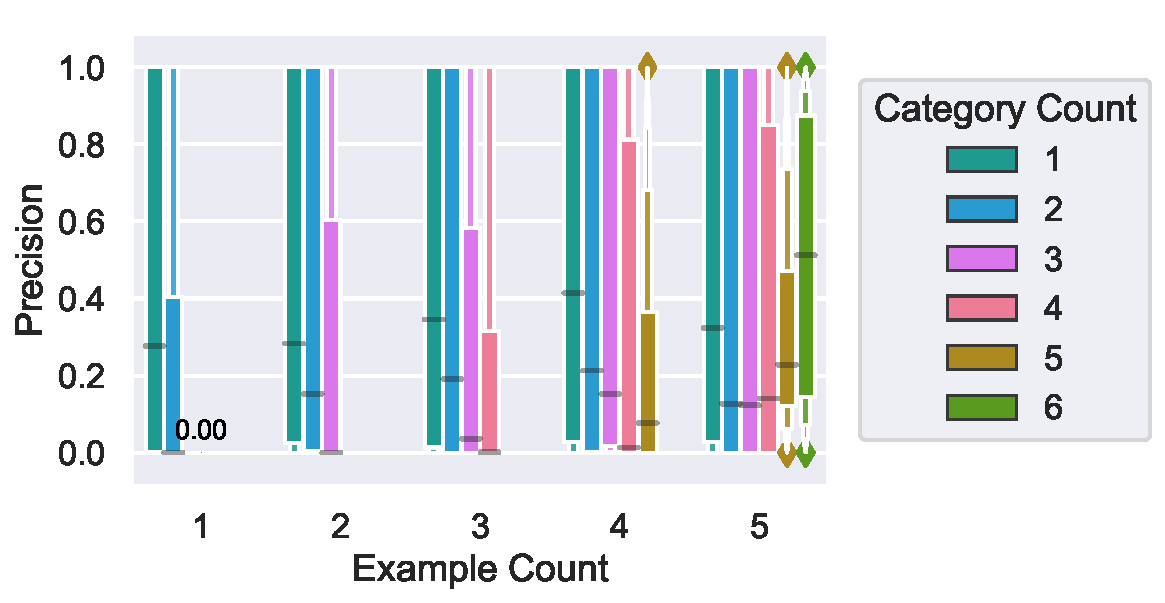
\includegraphics[width=\textwidth, clip]{img/big-study/precision-categorycount-examplecount-all.pdf}
		\caption{\todo{todo}}
		\label{fig:precision-categorycount-examplecount-all}
	\end{minipage}\hfill
	\begin{minipage}{0.45\textwidth}
		\centering
		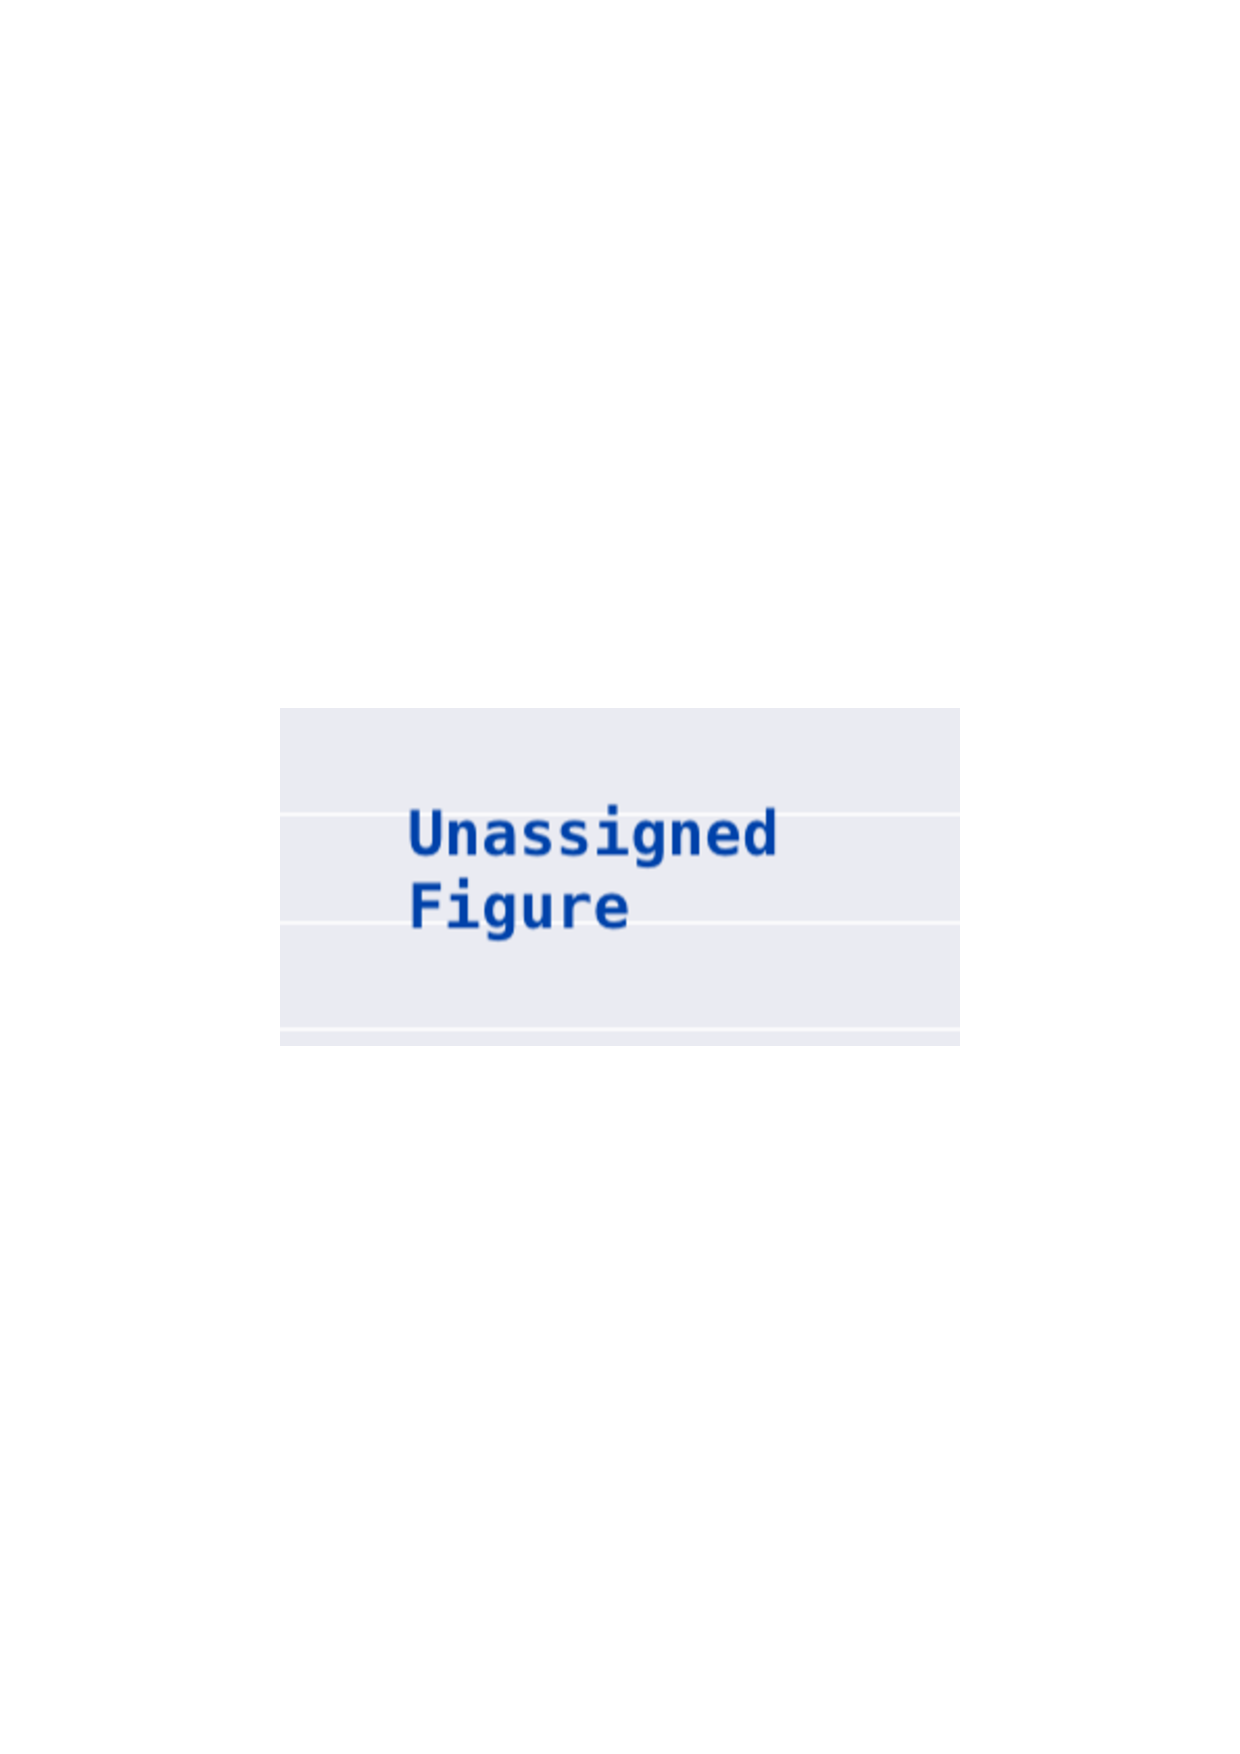
\includegraphics[width=\textwidth, clip]{img/big-study/xxx.pdf}
		\caption{\todo{todo}}
		\label{fig:xxx}
	\end{minipage}
\end{figure}

\subsubsection{Success-Rate}
\subsubsection{Precision}
\subsubsection{Example Categories}

\section{Discussion}
\todo{draw decision tree}

interpret results - when should PROSE be used? - when should text similarity be used? - when should keyword search be used? - answer RQ about PROSE \& other techniques
\section{Threats to Validity}

\end{document}
